\section*{Zielsetzung}
In diesem Versuch wurden kollodiale Halbleiter-Nanokristalle optisch zu Photolumineszenz angeregt und charakterisiert. Die elektronischen Eigenschaften, wie die Bandlücke wird bestimmt und die Abhängigkeit des Photolumineszenzlichtes von der Anregungslaserleistung, Polarisation und Anregungswellenlänge werden betrachtet.

\section{Theorie}
\subsection{Photolumineszenz}
    \begin{figure}[ht]
        \centering\captionsetup{format=plain}
        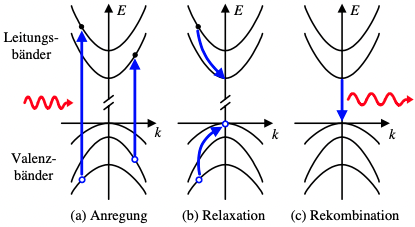
\includegraphics[width=0.5\textwidth]{bilder/PL_Grundschritte.png}
        \caption{Hier die drei grundlegenden Schritte zur Entstehung von Photolumineszenz in einem Halbleiter dargestellt. Entnommen aus \cite{Photolumineszenz}.}
        \label{fig:PL_Grundschritte}
    \end{figure}
    \FloatBarrier
    Photolumineszenz in Halbleitern tritt auf, wenn Elektronen im Valenzband über die Bandlücke in das Leitungsband angehoben werden, wie in \autoref{fig:PL_Grundschritte} a) zu sehen.
    Dies kann durch optische Anregung oder durch Injektion einer elektrischen Ladung passieren.
    Das angeregte Elektron lässt ein Loch im Valenzband zurück, welches über die Coulomb-Wechselwirkung mit dem Elektron gebunden ist.
    Es wird also effektiv ein Exziton erzeugt.
    Innerhalb einiger ps relaxieren das Elektron und das Loch an die Kanten ihrer Bänder durch nichtstrahlende Prozesse.
    Die Bandlücke stellt einen größeren Sprung in der Energie dar, sodass die spontane Emission eines Photons wahrscheinlicher ist und innerhalb weniger ns passiert.
    Dieser Übergang wird Rekombination genannt, da das Elektron in das Loch fällt und das Exziton vernichtet wird.
    
    Es gibt jedoch auch andere Arten von Exzitonen.
    Ist z.B. die Energie des Anregungslaser größer als die Bandlücke der Schale, werden Exzitonen in der Schale erzeugt und können von dem Kern eingefangen werden, wie in \autoref{fig:Exzitonen} a).
    Während der Relaxation eines Elektron-Loch-Paares, können weitere Exzitonen entstehen bzw. eingefangen werden.
    Die zusätzlichen Ladungsträger bewirken eine kleine Verschiebung der Rekombinationsenergie und somit des PL-Peaks.
    \autoref{fig:Exzitonen} c) zeigt einen Extremfall, der bei sehr hohen Anregungsintensitäten passieren kann.
    In diesem Fall ist der Zustand an der Leitungsbandkante noch von anderen Elektronen gefüllt, die noch nicht rekombiniert sind und es eröffnet sich die Möglichkeit, dass Elektronen-Loch-Paare auch aus höheren angeregten Zuständen rekombinieren können. 
    Es wird jedoch davon ausgegangen, dass die Beiträge der Exzitonenkomplexe zu vernachlässigen sind.
    \begin{figure}[ht]
        \centering\captionsetup{format=plain}
        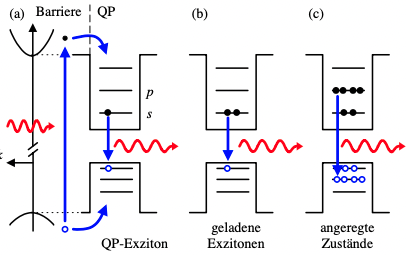
\includegraphics[width=0.5\textwidth]{bilder/Exzitonen.png}
        \caption{Hier sind verschiedene Arten von Exzitonen dargestellt. Entnommen aus \cite{Photolumineszenz}.}
        \label{fig:Exzitonen}
    \end{figure}
    % \FloatBarrier

\subsection{Halbleiter-Nanokristalle}
    Quantenpunkte machen die Untersuchung und Manipulation einzelner Strukturen auf der Nanoskala möglich, da ihre Eigenschaften durch ihre Größe, einige nm bis $\mu$m, bestimmt werden.
    \begin{figure}[ht]
        \centering\captionsetup{format=plain}
        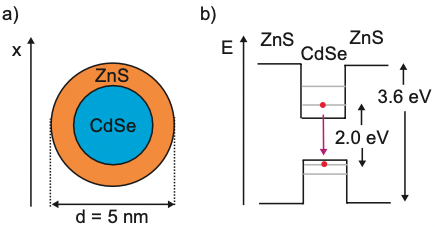
\includegraphics[width=0.5\textwidth]{bilder/Quantumdot.png}
        \caption{\textbf{a)} Der schematische Abbildung eines Kern-Schale-Quantenpunktes mit einem Kern aus CdSe und einer Schale aus ZnS. \textbf{b)} Die elektronische Struktur des Kern-Schale-Qunatenpunktes ist hier dargestellt. Entnommen aus \cite{anleitung}.}
        \label{fig:Quantumdot}
    \end{figure}
    \FloatBarrier
    Man betrachte einen kollodialen Halbleiter-Nanokristall mit einem Kern aus CdSe mit einer Bandlücke von \qty{1,74}{eV} und einer Schale aus ZnS mit einer Bandlücke von \qty{3,56}{eV} so wie in \autoref{fig:Quantumdot} zu dargestellt.
    Die Bandlücke der Schale ist größer als die des Kerns.
    Die Schale stellt also effektiv eine Potentialwand dar und der Kern ist der eigentliche Quantenpunkt.
    Diese Nanokristalle sind so klein, dass die Beweglichkeit der Ladungsträger auf der Größenskala ihrer De-Broglie-Wellenlänge einschränkt wird.
    Unter solchen Bedingungen passieren Quanteneffekte oder besser gesagt, eine Quantisierung der Energie tritt auf.
    Zur mathematischen Beschreibung der Quantenpunkte wird die Annahme getroffen, dass die Größe des Nanokristalls klein genug ist, um Quanteneffekte hervorzurufen, aber groß genug ist, dass im Inneren noch die periodische Festkörperstruktur erhalten ist.
    Die Wellenfunktion setzt sich somit zusammen aus einer Einhüllenden, die durch das einschließende Potential gegeben ist, der Bloch-Funktion und einer gitterperiodischen Funktion.

    Die Rekombinationsenergie $E_{\mathrm{R}}$ einzelner Exzitonen kann durch 
    \begin{equation}
        E_{\mathrm{R}} = E_{\mathrm{g}} + \frac{\hbar^2 \pi^2}{2 \mu a^2} - 1,786\, \frac{e^2}{4\pi \epsilon_0 \epsilon_r a} \qquad \mathrm{mit} \quad \mu = \frac{1}{m^*_{\mathrm{e}}} + \frac{1}{m^*_{\mathrm{h}}}
        \label{eqn:PL_formel}
    \end{equation}
    aproximiert werden.
    Beim ersten Summanden handelt es sich um die Bandlücke $E_{\mathrm{g}}$.
    Der zweite Term gibt die Energie des Elektrons in einem Quantenpunkt an.
    Die effektiven Massen in der reduzierten Masse $\mu$ berücksichtigt die Wechselwirkung des Exzitons mit dem Kristallfeld im Kern des Quantenpunktes.
    Der letzte Term bezieht die Coulomb-Wechselwirkung zwischen dem Elektron und dem zugehörigen Loch mit ein.
    
    Die Größe des Nanokristalls bestimmt also die energetische Struktur und ermöglicht die Floureszenzeigenschaften nach Belieben zu steuern, was in \autoref{fig:Groesse_zu_Farbe} dargestellt ist.
    \begin{figure}[ht]
        \centering\captionsetup{format=plain}
        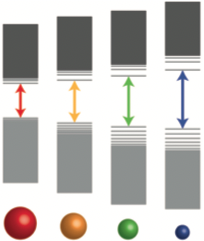
\includegraphics[width=0.3\textwidth]{bilder/Groesse_zu_Farbe.png}
        \caption{Die Größe der Quantenpunkte bestimmt die Wellenlänge des PL-Peaks. Entnommen aus \cite{Farben}.}
        \label{fig:Groesse_zu_Farbe}
    \end{figure}





